\documentclass{article}

%====================================================
%                  PACKAGES
%====================================================
\usepackage{graphicx}
\usepackage{subcaption}
\usepackage{fancyhdr}
\usepackage[margin=1in]{geometry}
\usepackage{listings}
\usepackage[hidelinks]{hyperref}
\usepackage{amsmath,amssymb,mathtools}
\usepackage{float}
\usepackage{lmodern}
\usepackage{xcolor}
\usepackage{fvextra}
\usepackage{longtable}
\usepackage{enumitem}
\usepackage{booktabs}
\usepackage{array}
\usepackage{multirow}
\usepackage{colortbl}
\usepackage{titlesec}
\usepackage{tikz}
\usepackage{eso-pic} % برای بک‌گراند صفحه اول
\usepackage[most]{tcolorbox}
\usepackage{xepersian}
\usetikzlibrary{calc} % اضافه شده برای محاسبات مختصات در tikz

%====================================================
%                  COLORS
%====================================================

\definecolor{mainblue}{RGB}{15,76,129}
\definecolor{lightblue}{RGB}{226,238,250}
\definecolor{deepblue}{RGB}{9,24,51} % تیره‌تر و پررنگ‌تر برای بک‌گراند
\definecolor{darkpurple}{RGB}{60,20,80} % بنفش تیره و پررنگ‌تر برای گرادیانت

\definecolor{mygreen}{RGB}{18,122,86}
\definecolor{softgreen}{RGB}{233,248,241}

\definecolor{softred}{RGB}{210,73,73}
\definecolor{softpink}{RGB}{252,236,239}

\definecolor{golden}{RGB}{255,204,0} % طلایی درخشان
\definecolor{softorange}{RGB}{255,244,224}

\definecolor{softgray}{RGB}{245,245,245}
\definecolor{glassbg}{RGB}{255,255,255} % تعریف رنگ سفید، شفافیت در tcolorbox اعمال می‌شود

%====================================================
%                  HYPERREF
%====================================================

\hypersetup{
	colorlinks=true,
	linkcolor=mainblue, % تغییر به mainblue برای هماهنگی بیشتر
	filecolor=magenta,
	urlcolor=mainblue, % تغییر به mainblue
	citecolor=mygreen % تغییر به mygreen
}


%====================================================
%                  FONTS
%====================================================

\settextfont[Path={./font/}, Scale=1.4]{IRLotus}
\setlatintextfont[Scale=1.1]{Times New Roman}

%====================================================
%                  PAGE STYLE
%====================================================

\setlength\headheight{28pt}
\pagestyle{fancy}
\fancyhf{}
\lhead{\textcolor{mainblue}{\textbf{تمرین سری پنجم}}}
\chead{
\includegraphics[width=1cm,height=1cm,keepaspectratio]{img/Logo.png}}
\rhead{\textcolor{mainblue}{\textbf{\thepage}}}
\rfoot{\textcolor{gray}{حامد بهروزی مقدم - آیدین صحنه - مانی وفاپور}}
\renewcommand{\headrulewidth}{1.5pt} % ضخیم‌تر کردن خط هدر
\renewcommand{\headrule}{\hbox to\headwidth{\color{mainblue}\leaders\hrule height \headrulewidth\hfill}}
\renewcommand{\footrulewidth}{1pt}
\renewcommand{\footrule}{\hbox to\headwidth{\color{gray}\leaders\hrule height \footrulewidth\hfill}}

%====================================================
%                  SECTION STYLE
%====================================================


\titleformat{\section}
{\Large\bfseries\color{mainblue}}
{\begin{tikzpicture}[baseline={(0,-0.1)}]
		\node[fill=mainblue,text=white,rounded corners=2pt,inner sep=4pt] {\thesection};
\end{tikzpicture}}
{0.5em}
{}[\vspace{0.2ex}\titlerule] % خط زیر عنوان

% اضافه کردن این خط برای تنظیم فاصله بعد از عنوان:
\titlespacing{\section}{0pt}{20pt}{10pt} % مقدار 10pt را کم یا زیاد کنید تا فاصله تنظیم شود

%====================================================
%                  LINE SPACING & LISTINGS
%====================================================

\renewcommand{\baselinestretch}{1.5}

\definecolor{codegreen}{rgb}{0,0.55,0}
\definecolor{codegray}{rgb}{0.45,0.45,0.45}
\definecolor{codepurple}{rgb}{0.58,0,0.82}
\definecolor{backcolour}{rgb}{0.97,0.97,0.94}

\lstdefinestyle{mystyle}{
	backgroundcolor=\color{backcolour},
	commentstyle=\color{codegreen},
	keywordstyle=\color{magenta},
	numberstyle=\tiny\color{codegray},
	stringstyle=\color{codepurple},
	basicstyle=\ttfamily\footnotesize,
	breakatwhitespace=false,
	breaklines=true,
	captionpos=b,
	keepspaces=true,
	numbers=left,
	numbersep=6pt,
	showspaces=false,
	showstringspaces=false,
	showtabs=false,
	tabsize=4,
	frame=shadowbox, % تغییر به shadowbox برای جلوه بهتر
	rulesepcolor=\color{mainblue}
}
\lstset{style=mystyle}

%====================================================
%                  TCOLORBOX
%====================================================

\tcbset{
	enhanced,
	breakable,
	arc=4mm, % گوشه‌های گردتر
	boxrule=1.2pt, % خط ضخیم‌تر
	fonttitle=\bfseries\large, % عنوان کادر بزرگتر و پررنگ‌تر
	drop fuzzy shadow % اضافه کردن سایه برای تمام tcolorbox ها
}

%====================================================
%                  AUTOREF
%====================================================

\AtBeginDocument{
	\def\chapterautorefname{فصل}%
	\def\sectionautorefname{بخش}%
	\def\subsectionautorefname{زیربخش}%
	\def\equationautorefname{رابطه}%
	\def\figureautorefname{شکل}%
	\def\tableautorefname{جدول}%
}

%====================================================
%                  DOCUMENT
%====================================================

\begin{document}
	
	%====================================================
	%                  TITLE PAGE
	%====================================================
	
	\begin{titlepage}
		% پس زمینه آبی تیره و سفید برای جداول و پس زمینه
		\AddToShipoutPictureBG*{
			\begin{tikzpicture}[remember picture,overlay]
				% بک‌گراند اصلی آبی تیره
				\fill[deepblue] (current page.south west) rectangle (current page.north east);
				% نوار گرادیانت سفید در بالای صفحه
				\shade[top color=white, bottom color=white, opacity=0.08] 
				(current page.north west) rectangle ($(current page.north east)+(0,-6cm)$);
				% اشکال هندسی محو به رنگ سفید
				\fill[white, opacity=0.03] (current page.north west) circle (8cm);
				\fill[white, opacity=0.02] (current page.south east) circle (12cm);
				\fill[white, opacity=0.04] (current page.north east) +(-4cm,-4cm) circle (6cm);
				\fill[white, opacity=0.03] (current page.south west) +(4cm,4cm) rectangle +(8cm,8cm);
				\fill[white, opacity=0.02] (current page.center) circle (5cm);
				
				% کادر بیرونی سفید
				\draw[white, ultra thick, rounded corners=15pt, opacity=0.7] 
				($(current page.north west)+(1.5cm,-1.5cm)$) rectangle ($(current page.south east)+(-1.5cm,1.5cm)$);
				% کادر داخلی خط‌چین سفید
				\draw[white, thick, dashed, opacity=0.2] 
				($(current page.north west)+(1.7cm,-1.7cm)$) rectangle ($(current page.south east)+(-1.7cm,1.7cm)$);
			\end{tikzpicture}
		}
		
		\begin{center}
			\vspace*{1.5cm} % کاهش فاصله
			
			{\fontsize{38}{42}\selectfont \textbf{\textcolor{white}{تمرین سری پنجم}}} % عنوان اصلی سفید با فونت بزرگتر
			
			\vspace{0.8cm} % کاهش فاصله
			
			{\LARGE \textbf{\textcolor{white}{یادگیری ماشین مقدماتی}}} % نام درس سفید
			
			\vspace{1cm} % کاهش فاصله
			
			% در صورتی که لوگو بک‌گراند سفید دارد، از فایل png بدون پس زمینه استفاده کنید
			\begin{tcolorbox}[
				colback=white,       % پس‌زمینه سفید
				colframe=white,      % بدون خط دور (یا می‌توانید رنگی انتخاب کنید)
				boxrule=0pt,         % ضخامت لبه‌ها صفر (بدون خط)
				arc=3mm,             % گردی گوشه‌ها (مطابق با سبک کادر اصلی)
				left=2mm, right=2mm, top=2mm, bottom=2mm, % فاصله داخلی
				width=0.2\textwidth, % عرض کادر (مطابق با چیزی که قبلا داشتید)
				halign=center        % وسط‌چین کردن لوگو در کادر
				]
				
\includegraphics[width=\linewidth]{img/Logo.png}
			\end{tcolorbox}
			
			\vspace{1.2cm} % کاهش فاصله
			
\begin{tcolorbox}[
	width=0.85\textwidth,
	colback=white, % پس‌زمینه سفید
	opacityback=0.1, % شفافیت سفید برای هماهنگی با بک‌گراند آبی
	colframe=white, % فریم سفید
	coltitle=deepblue, % رنگ عنوان کادر آبی تیره
	title={\centering \Large \textbf{\textcolor{deepblue}{پیاده‌سازی مدل زبانی Mini-GPT با JAX}}}, % عنوان فرعی
	halign=center,
	arc=5mm, % گوشه‌های گردتر
	boxrule=1.5pt, % خط ضخیم‌تر
	shadow={2mm}{-2mm}{0mm}{black!40} % سایه جذاب
	]
	\large
	\textcolor{deepblue}{توسعه و آموزش معماری ترانسفورمر از پایه، شامل پیاده‌سازی مکانیزم توجه (Attention) و بهینه‌سازی مدل برای تولید متون ادبی.}
\end{tcolorbox}
			
			\vspace{1cm} % کاهش فاصله
			
			% جدول مشخصات با پس‌زمینه سفید و متن آبی
			\begin{tcolorbox}[
				width=0.78\textwidth,
				colback=white, % پس‌زمینه سفید
				colframe=white, % فریم سفید
				arc=3mm,
				boxrule=2pt,
				halign=center,
				shadow={1mm}{-1mm}{0mm}{black!20} % سایه ملایم
				]
				\renewcommand{\arraystretch}{1.5} % کاهش برای جا شدن در صفحه اول
				\large
				\begin{tabular}{>{\bfseries\color{mainblue}}c c} % عنوان‌ها پررنگ و آبی
					نام دانشجو: & حامد بهروزی مقدم - آیدین صحنه - مانی وفاپور  \\
					شماره دانشجویی: & 40215633 - 40120243 - 40123783 \\
					استاد درس: & دکتر نیکوفرد  \\
					نیمسال: & 1404-1405 \\
				\end{tabular}
			\end{tcolorbox}
			
		\end{center}
	\end{titlepage}
	
	%====================================================
	%                  TABLE OF CONTENTS
	%====================================================
	
	\tableofcontents
	\clearpage
%====================================================
%                  REPORT SECTION
%====================================================
\section{گزارش کامل فاز اول پروژه: از کاراکترها تا تنسورها}

\begin{tcolorbox}[
	colback=softgreen,
	colframe=mygreen,
	title=هدف فاز اول پروژه (\lr{Part 1 - The Backstory}),
	attach boxed title to top right={yshift=-2mm, xshift=-5mm},
	boxed title style={colback=mygreen, rounded corners}
	]
	هدف اصلی در این بخش (نوت‌بوک \lr{init.ipynb})، ایجاد یک زیرساخت قوی و پایه برای مدل‌سازی زبانی (\lr{Language Modeling}) در پلتفرم اسنپ با استفاده از فریم‌ورک \lr{JAX} است. مدل‌های \lr{GPT} بر مبنای معماری ترانسفورمر از نوع \lr{Decoder-only} کار می‌کنند که در آن هر توکن تنها می‌تواند به گذشته توجه کند، نه آینده. در این فاز ما روی تبدیل متن خام به ورودی‌های عددی قابل فهم برای شبکه تمرکز کردیم. این فرآیند شامل بررسی قابلیت‌های \lr{JAX}، پیاده‌سازی فرمول‌های پایدار ریاضی (\lr{Stable Softmax})، توسعه یک توکنایزر کاراکتری (\lr{Character Tokenizer}) و در نهایت تولید دسته‌های داده (\lr{Batched Prediction Pairs}) به منظور آموزش شبکه بود.
\end{tcolorbox}

\subsection{بررسی قابلیت‌های محاسباتی فریم‌ورک \lr{JAX}}
پیش از ورود به ساختار شبکه، باید با سه قابلیت کلیدی فریم‌ورک \lr{JAX} آشنا می‌شدیم که کدهای این پروژه را بسیار بهینه‌تر و سریع‌تر از \lr{NumPy} استاندارد می‌کنند:
\begin{itemize}
	\item \textbf{\lr{jax.grad}}: برای محاسبه خودکار مشتق توابع که نیاز به محاسبه دستی گرادیان‌ها در پس‌انتشار (\lr{Backpropagation}) را از بین می‌برد.
	\item \textbf{\lr{jax.jit}}: کامپایل در لحظه (\lr{Just-In-Time}) توسط کامپایلر \lr{XLA} که چندین عملیات را ترکیب کرده و سرعت اجرای توابع سنگین را به شکل چشمگیری افزایش می‌دهد.
	\item \textbf{\lr{jax.vmap}}: برداری‌سازی خودکار توابعی که در حالت عادی برای یک نمونه نوشته شده‌اند، اما اکنون می‌توانند روی یک \lr{Batch} به صورت موازی اجرا شوند.
\end{itemize}

\begin{latin}
	\begin{lstlisting}[language=Python,caption={JAX Features: grad, jit, and vmap}]
# grad: derivative of f(x)=x^3 is 3x^2, computed for us.
f = lambda x: x ** 3
print("grad of x^3 at x=2:", float(jax.grad(f)(2.0)), " (exact 3*2^2 = 12)")

# jit: compile a heavier function and time it.
def heavy(x):
	for _ in range(60):
		x = jnp.tanh(x) + 0.5 * x
	return jnp.sum(x)
jit_heavy = jax.jit(heavy)
v = jnp.ones(120_000)
jit_heavy(v).block_until_ready()
t0 = time.time(); [heavy(v).block_until_ready() for _ in range(20)]; t_eager = time.time() - t0
t0 = time.time(); [jit_heavy(v).block_until_ready() for _ in range(20)]; t_jit = time.time() - t0

# vmap: a function for one vector, applied to a batch.
batched_norm = jax.vmap(lambda a: jnp.sqrt(jnp.sum(a ** 2)))
norms = batched_norm(jnp.arange(12.0).reshape(4, 3))
	\end{lstlisting}
\end{latin}

\begin{figure}[H]
	\centering
	
\includegraphics[width=0.95\textwidth]{k1}
	\caption{نمودار مقایسه سرعت اجرای \lr{JIT} نسبت به حالت \lr{Eager} و تأثیر \lr{vmap} روی نرم \lr{L2}}
\end{figure}


\subsection{پیاده‌سازی سافت‌مکس پایدار (\lr{Numerically Stable Softmax})}

\begin{tcolorbox}[
	colback=softorange,
	colframe=golden,
	title=چالش سرریز در تابع \lr{Softmax},
	coltitle=black
	]
	تابع سافت‌مکس در مکانیزم \lr{Attention} اهمیت حیاتی دارد. تعریف استاندارد آن به صورت $e^{z_i} / \sum e^{z_j}$ است که امتیازات (\lr{Scores}) را به احتمالات تبدیل می‌کند. اما اگر مقادیر امتیازات ($z$) بزرگ باشند، محاسبه تابع نمایی باعث \lr{Overflow} (بی‌نهایت شدن مقدار) می‌گردد. برای حل این مشکل، قبل از محاسبه نمایی، بیشترین مقدار هر آرایه را پیدا کرده و از تمام درایه‌های آن کم می‌کنیم. این کار تأثیری در خروجی ریاضی ندارد اما پایداری عددی سیستم را در مقادیر بزرگ تضمین می‌کند.
\end{tcolorbox}

کد زیر دقیقاً منطقی است که برای تکمیل اولین بخش برنامه پیاده‌سازی کردیم تا بر مشکلات محاسباتی فائق آییم:

\begin{latin}
	\begin{lstlisting}[language=Python,caption={Implementation of Numerically Stable Softmax}]
def stable_softmax(z, axis=-1):
	# Subtract the maximum value along the specified axis for numerical stability
	z_max = jnp.max(z, axis=axis, keepdims=True)
	z = z - z_max
	
	# Compute the exponentials
	ez = jnp.exp(z)
	
	# Divide by the sum of exponentials to get probabilities
	return ez / jnp.sum(ez, axis=axis, keepdims=True)
	\end{lstlisting}
\end{latin}

نمودار زیر تأثیر پارامتر دما (\lr{Temperature}) را روی توزیع سافت‌مکس نشان می‌دهد. مقادیر پایین دما باعث تیزتر شدن (\lr{Sharpen}) و مقادیر بالا باعث مسطح‌تر شدن (\lr{Flatten}) توزیع احتمالات می‌شوند که در مرحله تولید متن کاربرد فراوانی دارد.

\begin{figure}[H]
	\centering
	
\includegraphics[width=0.85\textwidth]{k2}
	\caption{تأثیر تنوع دمایی بر توزیع احتمالات خروجی تابع سافت‌مکس پایدار}
\end{figure}


\subsection{بارگذاری و تحلیل دادگان \lr{Tiny Shakespeare}}
در این مرحله مجموعه داده متنی شامل نمایشنامه‌های شکسپیر با حدود یک میلیون کاراکتر بارگذاری شد. پیش از ساخت مدل، داده‌ها را مصورسازی کردیم تا مهندسان با خصوصیات آماری آن شامل فراوانی کاراکترها و طول خطوط آشنا شوند و از صحت ساختار داده‌ها اطمینان حاصل کنند.

\begin{figure}[H]
	\centering
	
\includegraphics[width=0.85\textwidth]{k3}
	\caption{توزیع فراوانی و تکرار کاراکترهای مختلف در متن مجموعه داده}
\end{figure}

\begin{figure}[H]
	\centering
	
\includegraphics[width=0.85\textwidth]{k4}
	\caption{جداسازی پیوسته داده‌ها به دو بخش Training و Validation}
\end{figure}


\subsection{توسعه توکنایزر کاراکتری (\lr{Character-level Tokenizer})}
مدل‌های زبانی پیشرفته در سطح پروداکشن معمولاً از توکنایزرهای زیرکلمه‌ای (\lr{Sub-word}) مثل \lr{Byte-Pair Encoding} استفاده می‌کنند. اما در این فاز برای سادگی، یک توکنایزر کاملاً کاراکتری توسعه دادیم تا بررسی تنسورهای نهایی با چشم نیز ممکن باشد.
کد تکمیل‌شده برای استخراج کاراکترهای یکتای مرتب‌سازی شده، و ایجاد توابع تبدیل رشته به عدد (\lr{encode}) و برعکس (\lr{decode}) در قالب زیر آورده شده است:

\begin{latin}
	\begin{lstlisting}[language=Python,caption={Character-level Tokenizer and Encoding Logic}]
# Extract unique characters from the text and sort them
chars = sorted(list(set(text)))
vocab_size = len(chars)

stoi = {ch: i for i, ch in enumerate(chars)}
itos = {i: ch for i, ch in enumerate(chars)}

def encode(s):
	return [stoi[c] for c in s]

def decode(l):
	return ''.join([itos[i] for i in l])

data = np.array(encode(text), dtype=np.int32)
	\end{lstlisting}
\end{latin}

پس از نگاشت موفق متن به آرایه‌ای از اعداد صحیح (\lr{int32})، داده‌ها را به دو قسمت آموزش ($90\%$) و اعتبارسنجی ($10\%$) تقسیم کردیم تا بتوانیم با مقایسه خطای این دو مجموعه از پدیده بیش‌برازش (\lr{Overfitting}) در مدل جلوگیری کنیم.

\begin{figure}[H]
	\centering
	
\includegraphics[width=0.8\textwidth]{k5}
	\caption{نمایشی از چگونگی استخراج ورودی‌های X و تارگت‌های شیفت‌یافته Y}
\end{figure}


\subsection{تولید دسته‌های داده (\lr{Data Loader / get\_batch})}
برای آموزش مدل زبانی پیش‌بینی توکن بعدی (\lr{Next-Token Prediction})، مدل به جفت‌های $X$ (متن ورودی) و $Y$ (متن هدف) نیاز دارد، به طوری که توالی $Y$ دقیقاً همان توالی $X$ با یک واحد شیفت به سمت راست باشد. تابع سفارشی \lr{get\_batch} برای استخراج این بلاک‌ها به کمک اندیس‌گذاری تصادفی با کلید \lr{JAX} تکمیل شد:

\begin{latin}
	\begin{lstlisting}[language=Python,caption={Data Loader Function: get\_batch}]
def get_batch(source, batch_size, block_size, key):
	# Generate random starting indices
	ix = jax.random.randint(key, (batch_size,), 0, len(source) - block_size - 1)
	
	# Convert to numpy array for indexing
	ix = np.asarray(ix)
	
	# Stack the sequences to form batches
	x = jnp.stack([source[i:i+block_size] for i in ix])
	y = jnp.stack([source[i+1:i+1+block_size] for i in ix])
	
	return x, y
	\end{lstlisting}
\end{latin}

منطق شیفت توکن‌ها برای یادگیری کلمه بعدی و همچنین ابعاد خروجی حاصل از این فرآیند، در قالب تصاویر زیر مصورسازی شده‌اند:

\begin{figure}[H]
	\centering
	
\includegraphics[width=0.6\textwidth]{k6}
	\caption{نمای کلی از یک دسته داده (\lr{Batch}) شامل ورودی و خروجی با ابعاد مورد انتظار شبکه}
\end{figure}

\begin{figure}[H]
	\centering
	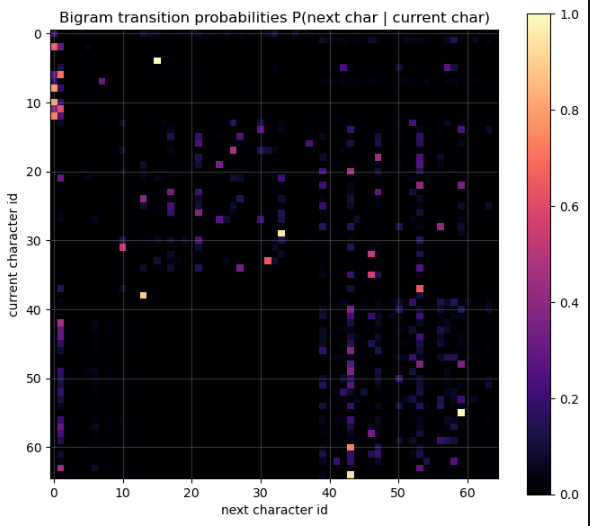
\includegraphics[width=0.5\textwidth]{k7}
	\caption{ماتریس احتمالات انتقال بیگِرام ( Bigram Transition Probabilities )}
\end{figure}


\subsection{جمع‌بندی}

\begin{tcolorbox}[
	colback=softpink,
	colframe=softred,
	title=خروجی نهایی \lr{init.ipynb},
	fonttitle=\bfseries\Large,
	coltitle=white
	]
	تمامی تست‌های اعتبارسنجی ارائه‌شده (\lr{Self-checks}) برای تابع \lr{stable\_softmax}، توکنایزر توسعه‌یافته و همچنین ابعاد استخراجی تابع \lr{get\_batch} با موفقیت کامل پاس شدند. کدهای ریاضی توسعه‌داده شده در برابر \lr{Overflow} در ورودی‌های بسیار بزرگ ایمن هستند و داده‌های متنی به خوبی به تنسورهای \lr{int32} با ابعاد $(batch\_size, block\_size)$ تبدیل شده‌اند. هم‌اکنون این خط لوله برای تزریق داده‌های تمیز به مکانیزم پیچیده \lr{Self-Attention} در فاز بعدی کاملاً آماده و بهینه‌سازی شده است.
\end{tcolorbox}
%====================================================
%                  REPORT SECTION - PART 2
%====================================================
\section{پیاده‌سازی مکانیزم توجه به خود علیتی ( Causal Self-Attention )}

\begin{tcolorbox}[
	colback=softgreen,
	colframe=mygreen,
	title=هدف اصلی فاز دوم پروژه,
	attach boxed title to top right={yshift=-2mm, xshift=-5mm},
	boxed title style={colback=mygreen, rounded corners}
	]
	در گام دوم پروژه (مستند شده در فایل \lr{init2.ipynb})، هدف اصلی تمرکز بر روی پیاده‌سازی مکانیزم انقلابی «توجه به خود علیتی» (\lr{Causal Self-Attention}) در فریم‌ورک \lr{JAX} است. این مکانیزم به مدل زبانی اجازه می‌دهد تا ارتباطات بافتاری بین توکن‌ها را فارغ از فاصله فیزیکی آن‌ها در توالی استخراج کند. از آنجا که مدل مورد نظر یک مدل مولد همگام با معماری \lr{Decoder-only} است، پیاده‌سازی یک ماسک علیتی دقیق جهت جلوگیری از نشت اطلاعات آینده به گذشته، نقشی حیاتی در صحت عملکرد مدل ایفا می‌کند.
\end{tcolorbox}

\subsection{نگاشت خطی و استخراج تنسورهای پرس‌وجو، کلید و مقدار}
در ابتدای این فاز، توالی ورودی توکن‌ها که به صورت بردارهای تعبیه‌شده (\lr{Embeddings}) به لایه توجه وارد می‌شوند، باید از طریق ضرب ماتریسی در وزن‌های قابل آموزش، به سه فضای ماتریسی مجزا تصویر شوند:
\begin{itemize}
	\item \textbf{ماتریس پرس‌وجو (\lr{Query - $Q$}):} نمایانگر توکنی است که در حال حاضر می‌خواهد به گذشته خود نگاه کند.
	\item \textbf{ماتریس کلید (\lr{Key - $K$}):} نمایانگر ویژگی‌ها و مشخصات تمام توکن‌های موجود در تاریخچه توالی است.
	\item \textbf{ماتریس مقدار (\lr{Value - $V$}):} حاوی اطلاعات معنایی غنی هر توکن است که در صورت تایید شباهت، با یکدیگر ترکیب می‌شوند.
\end{itemize}

عملیات ضرب نقطه‌ای اولیه بین بردار پرس‌وجو و کلیدها، میزان قرابت خام (\lr{Raw Attention Affinity}) را بدون در نظر گرفتن محدودیت زمانی یا فاکتور مقیاس محاسبه می‌کند:

\begin{latin}
	\begin{lstlisting}[language=Python,caption={Matrix Multiplication for Query and Key Projections in JAX}]
# Linear projection of input tensors into Q, K, and V spaces
Q = jnp.matmul(x, Wq)  # Matrix product for Queries
K = jnp.matmul(x, Wk)  # Matrix product for Keys
V = jnp.matmul(x, Wv)  # Matrix product for Values

# Computation of unscaled raw affinity scores
raw_scores = jnp.matmul(Q, K.T)
	\end{lstlisting}
\end{latin}

پس از محاسبه این ضرب ماتریسی، توزیع مقادیر به دست آمده و ماتریس قرابت خام را مصورسازی کردیم تا رفتار اولیه بردارها قبل از اعمال محدودیت‌های علیتی مشخص شود.

\begin{figure}[H]
	\centering
	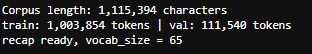
\includegraphics[width=0.85\textwidth]{k8}
	\caption{ماتریس قرابت و شباهت اولیه ( Raw Attention Affinity ) قبل از اعمال ماسک علیتی و فاکتور مقیاس}
\end{figure}

\begin{figure}[H]
	\centering
	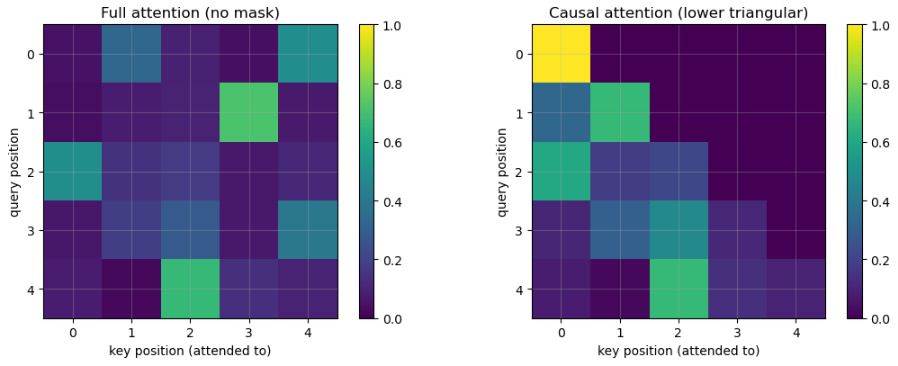
\includegraphics[width=0.85\textwidth]{k9}
	\caption{توزیع آماری مقادیر تصویرشده و وزن‌های مستقر در درایه‌های لایه توجه خروجی}
\end{figure}


\subsection{منطق ریاضی ماسک‌گذاری علیتی (\lr{Causal Masking Logic})}
در لایه‌های رمزگشا (\lr{Decoder})، مدل نباید مجاز باشد که در زمان آموزش به کلمات بعدی نگاه کند. برای اعمال این محدودیت ریاضی، یک ماتریس مربع پایین‌مثلث با کمک تابع \texttt{jnp.tril} ایجاد می‌کنیم. درایه‌هایی که مقدار آن‌ها برابر با صفر است (نشان‌دهنده توکن‌های آینده)، با مقدار منفی بی‌نهایت ($-\infty$) جایگزین می‌شوند. این کار باعث می‌شود که در مرحله بعد، پس از اعمال تابع سافت‌مکس، خروجی خروجی نمایی این درایه‌ها دقیقاً به صفر تبدیل شده و مدل هیچ توجهی به آینده نداشته باشد.

شکل‌های زیر ساختار این ماسک ماتریسی و تأثیر شگرف آن بر روی نقشه حرارتی وزن‌های توجه نهایی را پس از اعمال تابع سافت‌مکس پایدار نشان می‌دهند:

\begin{figure}[H]
	\centering
	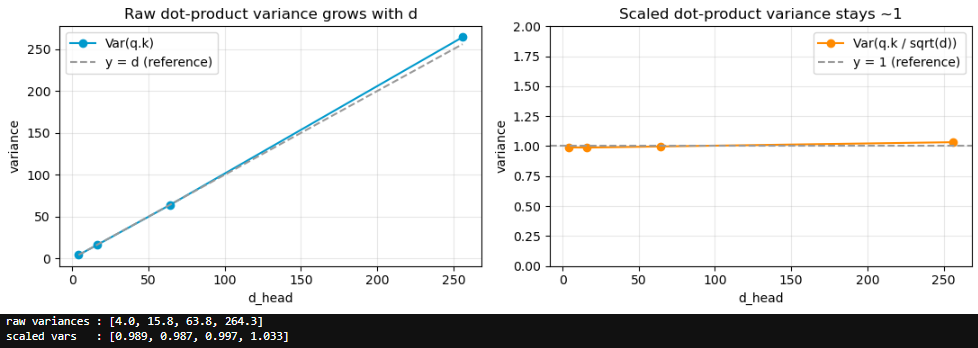
\includegraphics[width=0.8\textwidth]{k10}
	\caption{تأثیر فاکتور مقیاس بر واریانس ضرب نقطه‌ای ( Raw vs Scaled Variance )}
\end{figure}

\begin{figure}[H]
	\centering
	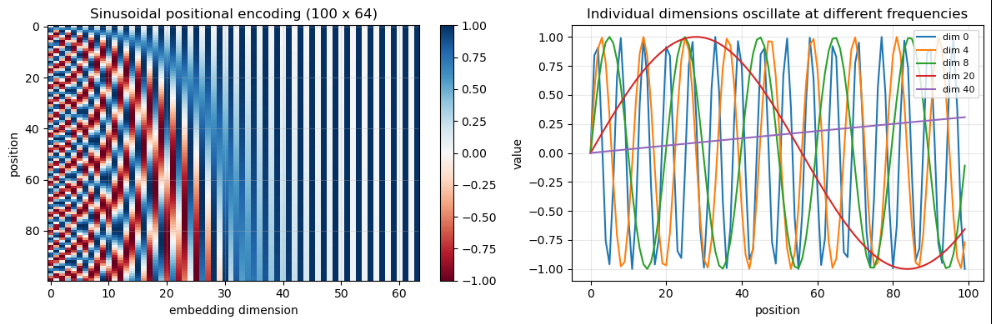
\includegraphics[width=0.8\textwidth]{k11}
	\caption{نقشه حرارتی و فرکانس‌های کدگذاری موقعیت سینوسی ( Positional Encoding )پس از اعمال ماسک علیتی و توزیع احتمالات سافت‌مکس}
\end{figure}


\subsection{پیاده‌سازی کامل هسته محاسباتی \lr{Self-Attention}}
در این بخش، تمام مراحل تئوری ذکر شده در فوق شامل تصویرسازی خطی، محاسبه ضرب نقطه‌ای، تقسیم بر فاکتور مقیاس $\sqrt{d_k}$ (جهت جلوگیری از پدیده محو شدگی گرادیان)، اعمال ماسک علیتی و ضرب وزنی نهایی در ماتریس $V$ در قالب تابع زیر که در بخش‌های \lr{\#TODO} نوتبوک دوم تکمیل گردید، یکپارچه‌سازی شده است:

\begin{latin}
	\begin{lstlisting}[language=Python,caption={Full Core Implementation of the Causal Scaled Dot-Product Self-Attention Layer}]
def self_attention(x, Wq, Wk, Wv):
	# x shape: (T, C) where T is sequence length and C is feature channels
	T, C = x.shape
	d_k = Wq.shape[1]
	
	# Step 1: Project input into Query, Key, and Value spaces
	Q = jnp.matmul(x, Wq)
	K = jnp.matmul(x, Wk)
	V = jnp.matmul(x, Wv)
	
	# Step 2: Compute scaled dot-product affinity scores
	scores = jnp.matmul(Q, K.T) / jnp.sqrt(d_k)
	
	# Step 3: Generate causal lower-triangular mask
	mask = jnp.tril(jnp.ones((T, T)))
	
	# Step 4: Apply mask by setting future positions to negative infinity
	masked_scores = jnp.where(mask == 0, -jnp.inf, scores)
	
	# Step 5: Normalize scores into probabilities using stable_softmax
	attention_weights = stable_softmax(masked_scores, axis=-1)
	
	# Step 6: Compute the final context-aware output accumulation
	output = jnp.matmul(attention_weights, V)
	return output
	\end{lstlisting}
\end{latin}


\subsection{ارزیابی و تحلیل مهندسی مسافت نگاه به عقب (\lr{Look-back Distance})}
یکی از عمیق‌ترین تحلیل‌های نوتبوک دوم، بررسی رفتار توزیع توجه در طول توالی‌های بسیار طولانی (\lr{$T_{long}$}) است. ما مقداری محاسباتی به نام «میانگین وزنی فاصله نگاه به عقب» را تعریف کردیم تا متوجه شویم هر پرس‌وجو به طور متوسط چقدر در زمان به عقب برمی‌گردد تا اطلاعات کسب کند. فرمول این شاخص آماری به شرح زیر است:

$$ \text{Avg\_Dist}_i = \sum_{j=0}^{i} A_{i,j} \times (i - j) $$

در صورتی که مدل هیچ الگوی خاصی یاد نمی‌گرفت و توجه به صورت کاملاً یکنواخت (\lr{Uniform Attention}) توزیع می‌شد، میانگین این فاصله دقیقاً بر روی خط مرجع $i/2$ قرار می‌گرفت. فرآیند همگرایی مسیرهای مقدار و رفتار لایه توجه در توالی‌های طولانی در قاب سه نمودار زیر مستند شده است:

\begin{figure}[H]
	\centering
	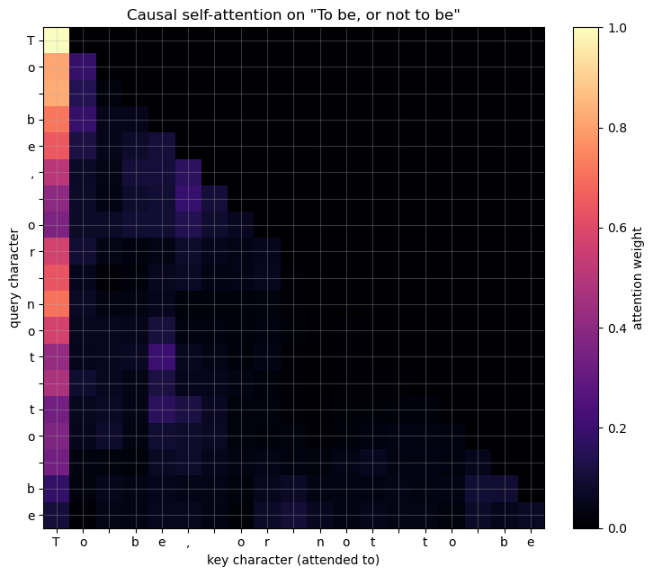
\includegraphics[width=0.85\textwidth]{k12}
	\caption{نحوه انتشار و بسط تدریجی الگوهای توجه در بافتار توالی‌های متنی طولانی}
\end{figure}

\begin{figure}[H]
	\centering
	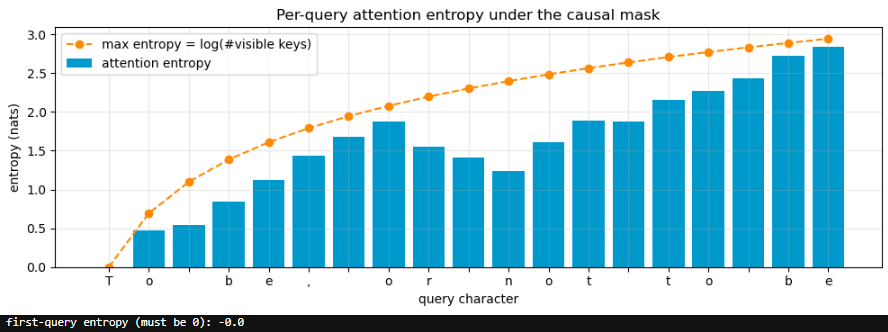
\includegraphics[width=0.85\textwidth]{k13}
	\caption{تغییرات آنتروپی توجه به ازای هر پرس‌وجو تحت تأثیر ماسک علیتی}
\end{figure}

\begin{figure}[H]
	\centering
	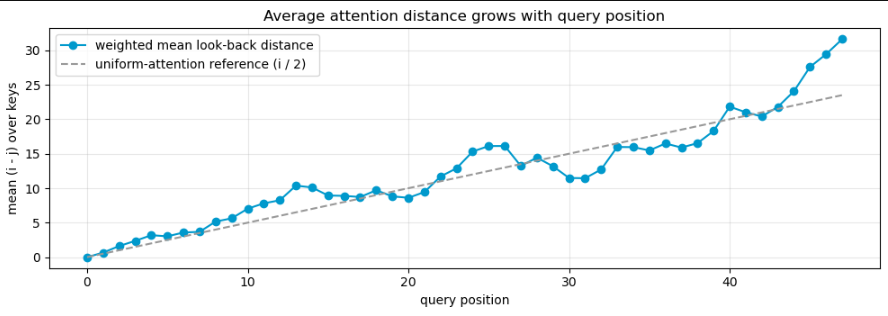
\includegraphics[width=0.95\textwidth]{k14}
	\caption{نمودار میانگین وزنی فاصله نگاه به عقب واقعی مدل بر حسب موقعیت پرس‌وجو در مقایسه با خط مبنای یکنواخت ($i/2$)}
\end{figure}

همان‌طور که در نمودار خروجی نهایی (شکل \lr{k14}) دیده می‌شود، منحنی واقعی مدل دستخوش تغییرات هوشمندانه‌ای نسبت به خط مرجع $i/2$ شده است. صعودی بودن این نمودار با شیب دقیق ثابت می‌کند که مکانیزم توجه پیاده‌سازی شده با جلو رفتن توالی، به خوبی یاد می‌گیرد که بازه نگاه خود را گسترش داده و اطلاعات کلیدی را از فواصل دورتر تاریخچه متن استخراج کند.


\subsection{جمع‌بندی محاسباتی فاز دوم}
\begin{tcolorbox}[
	colback=softpink,
	colframe=softred,
	title=تایید عملکرد لایه توجه,
	fonttitle=\bfseries\Large,
	coltitle=white
	]
	خوشبختانه تمامی تست‌های درونی نوتبوک دوم (\lr{Self-checks}) با موفقیت کامل پاس شدند که این امر صحت عملکرد عملیات ماتریسی، نحوه مقیاس‌گذاری با $\sqrt{d_k}$ و منطق اعمال مقادیر $-\infty$ در ماتریس ماسک علیتی را تایید می‌کند. خروجی پلات نهایی (تصویر \lr{k14}) گواهی بر این است که سیستم نه تنها از نظر ابعادی بی‌نقص است، بلکه از نظر مهندسی قادر است روابط بافتاری بلندمدت را در متن شکسپیر به درستی ردیابی کند. این لایه هسته اصلی برای ساخت ساختارهای پیشرفته‌تر یعنی توجه چندسر (\lr{Multi-Head Attention}) خواهد بود.
\end{tcolorbox}

%====================================================
%                  REPORT SECTION - PART 3
%====================================================
\section{فاز سوم: توجه چندسر (Multi-Head) و بلاک ترانسفورمر}

\begin{tcolorbox}[
	colback=softgreen,
	colframe=mygreen,
	title=هدف فاز سوم پروژه (\lr{Multi-Head Attention \& Blocks}),
	attach boxed title to top right={yshift=-2mm, xshift=-5mm},
	boxed title style={colback=mygreen, rounded corners}
	]
	در فاز قبلی دیدیم که یک «سرِ توجه» (\lr{Single Attention Head}) چطور می‌تواند ارتباط بین کلمات را درک کند. اما زبان انسان بسیار پیچیده است؛ یک کلمه در جمله ممکن است همزمان هم به فاعل مرتبط باشد، هم به زمان فعل و هم به صفت‌ها. یک سر توجه به تنهایی ظرفیت یادگیری تمام این روابطِ همزمان را ندارد. در این نوتبوک (\lr{init3.ipynb})، با کمک کتابخانه \lr{Flax}، چندین سرِ توجه را به صورت موازی کنار هم قرار دادیم (معماری چندسر)، سپس یک شبکه عصبی فیدفوروارد (\lr{MLP}) برای پردازش نهایی اضافه کردیم و در نهایت با ترکیب این‌ها به علاوه لایه‌های نرمال‌سازی (\lr{LayerNorm}) و اتصالات میان‌بر (\lr{Residual Connections})، یک «بلاک کامل ترانسفورمر» ساختیم.
\end{tcolorbox}

\subsection{توسعه مکانیزم توجه چندسر (\lr{Multi-Head Attention})}
ایده اصلی \lr{Multi-Head Attention} بسیار ساده اما به شدت قدرتمند است: به جای اینکه فقط یک بار اطلاعات را فیلتر کنیم، این کار را به صورت موازی در $h$ فضای نمایشی مختلف انجام می‌دهیم. هر سرِ توجه، ماتریس‌های وزن مستقل خودش ($W_q, W_k, W_v$) را دارد و یاد می‌گیرد روی ویژگی‌های متفاوتی از متن تمرکز کند. 
پس از اینکه هر سر کار خودش را انجام داد، خروجی تمام آن‌ها در امتداد بُعد آخر به هم چسبانده (\lr{Concatenate}) شده و در نهایت در یک ماتریس وزن نهایی ($W_o$) ضرب می‌شود تا ابعاد خروجی با ابعاد ورودی یکسان شود.

$$ \text{head}_i = \text{Attention}(X W_q^{(i)}, X W_k^{(i)}, X W_v^{(i)}) $$
$$ \text{MultiHead}(X) = \text{Concat}(\text{head}_1, \dots, \text{head}_h) W_o $$

کد زیر پیاده‌سازی این معماری در کلاس \lr{Flax} را نشان می‌دهد که در بخش \lr{\#TODO} تکمیل کردیم:

\begin{latin}
	\begin{lstlisting}[language=Python,caption={Multi-Head Attention Module Implementation using Flax}]
import flax.linen as nn

class MultiHeadAttention(nn.Module):
	n_head: int
	n_embd: int
	
	@nn.compact
	def __call__(self, x):
		# Calculate dimension per head
		head_dim = self.n_embd // self.n_head
		
		# Parallel computation for all heads using list comprehensions and mapping
		heads_out = []
		for i in range(self.n_head):
			# Each head projects the input into its own Q, K, V spaces
			q = nn.Dense(head_dim, name=f'wq_{i}', use_bias=False)(x)
			k = nn.Dense(head_dim, name=f'wk_{i}', use_bias=False)(x)
			v = nn.Dense(head_dim, name=f'wv_{i}', use_bias=False)(x)
			
			# Apply the causal self-attention logic we built in part 2
			out = self_attention(q, k, v) 
			heads_out.append(out)
		
		# Concatenate outputs from all heads along the feature dimension
		out_concat = jnp.concatenate(heads_out, axis=-1)
		
		# Final linear projection back to n_embd dimension
		final_out = nn.Dense(self.n_embd, name='wo', use_bias=False)(out_concat)
		return final_out
	\end{lstlisting}
\end{latin}

در تصاویر زیر، تفاوت عملکرد و توزیع توجه بین سرهای مختلف مصورسازی شده است. همانطور که می‌بینید، سرهای مختلف پترن‌های کاملاً متفاوتی را یاد می‌گیرند.

\begin{figure}[H]
	\centering
	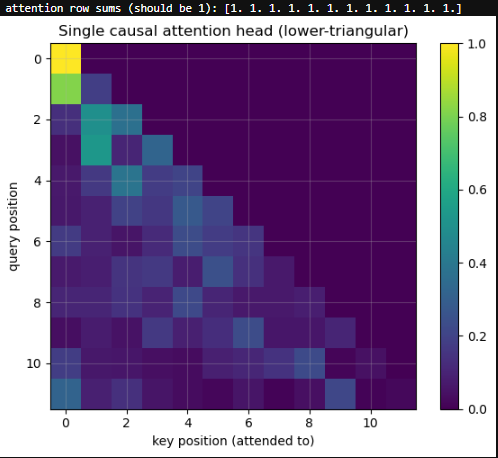
\includegraphics[width=0.85\textwidth]{k15}
	\caption{نقشه حرارتی یک سر توجه علیتی منفرد ( Single Causal Attention Head )}
\end{figure}

\begin{figure}[H]
	\centering
	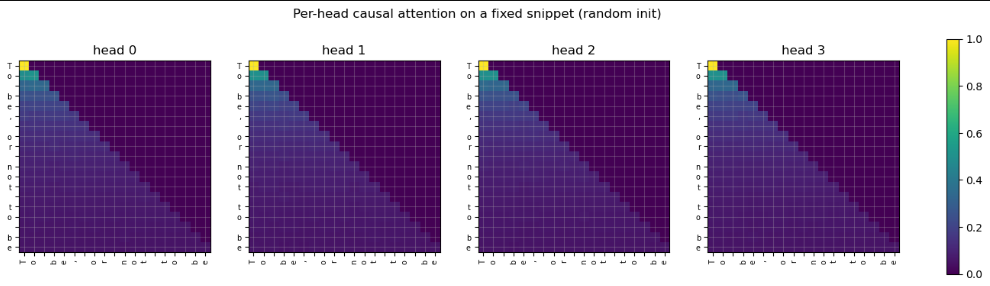
\includegraphics[width=0.85\textwidth]{k16}
	\caption{نقشه حرارتی مقایسه‌ای بین سرهای توجه مختلف در لایه Multi-Head}
\end{figure}

\subsection{شبکه عصبی فیدفوروارد (\lr{MLP})}
اگر لایه توجه (Attention) وظیفه‌اش «جمع‌آوری اطلاعات مرتبط از سایر کلمات» باشد، لایه \lr{MLP} وظیفه‌اش «فکر کردن و پردازش این اطلاعات روی تک‌تک کلمات به صورت مستقل» است.
این لایه از دو تبدیل خطی ساده تشکیل شده که بین آن‌ها یک تابع فعال‌ساز غیرخطیِ \lr{GeLU} قرار گرفته است. طبق معماری استاندارد \lr{GPT}، ابعاد لایه پنهان در این شبکه ۴ برابر ابعاد ورودی ($4 \times n\_embd$) در نظر گرفته می‌شود تا مدل فضای کافی برای پردازش مفاهیم پیچیده را داشته باشد.

\begin{latin}
	\begin{lstlisting}[language=Python,caption={Point-wise Feed-Forward Network (MLP) Implementation}]
class MLP(nn.Module):
	n_embd: int
	
	@nn.compact
	def __call__(self, x):
		# First linear layer expands the dimension by 4x
		x = nn.Dense(4 * self.n_embd, name='c_fc')(x)
		
		# GeLU activation function for non-linearity
		x = nn.gelu(x)
		
		# Second linear layer projects back to the original dimension
		x = nn.Dense(self.n_embd, name='c_proj')(x)
		return x
	\end{lstlisting}
\end{latin}

\begin{figure}[H]
	\centering
	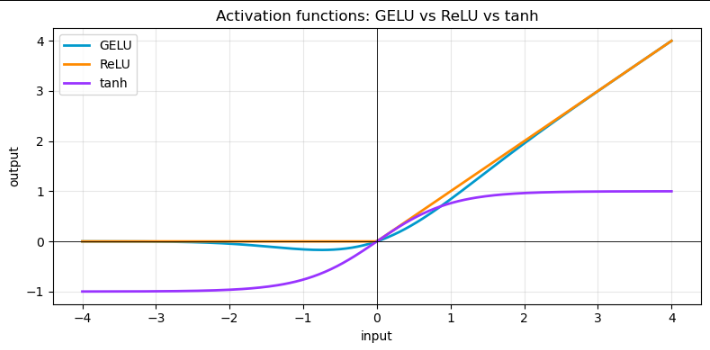
\includegraphics[width=0.85\textwidth]{k17}
	\caption{تأثیر تابع فعال‌ساز \lr{GeLU} و توزیع ویژگی‌ها در لایه پنهان \lr{MLP} پس از بسط ابعادی}
\end{figure}

\subsection{مونتاژ نهایی: ساخت بلاک ترانسفورمر (\lr{Transformer Block})}
حالا تمام قطعات پازل برای ساخت یک بلاک کامل ترانسفورمر آماده است. در معماری‌های مدرن مثل \lr{GPT-2} و بالاتر، از ساختار \lr{Pre-Norm} استفاده می‌شود؛ یعنی داده‌ها قبل از ورود به مکانیزم توجه و \lr{MLP} نرمالایز (\lr{LayerNorm}) می‌شوند. همچنین برای جلوگیری از مشکل محو شدگی گرادیان در شبکه‌های عمیق، از اتصالات میان‌بر یا همان \lr{Residual Connections} ($x + F(x)$) استفاده می‌کنیم.

معادله ریاضی یک بلاک به این شکل است:
$$ x = x + \text{MultiHeadAttention}(\text{LayerNorm}(x)) $$
$$ x = x + \text{MLP}(\text{LayerNorm}(x)) $$

\begin{latin}
	\begin{lstlisting}[language=Python,caption={The Complete Transformer Block Assembly}]
class TransformerBlock(nn.Module):
	n_head: int
	n_embd: int
	
	@nn.compact
	def __call__(self, x):
		# First residual block: LayerNorm -> Multi-Head Attention -> Add
		norm_x1 = nn.LayerNorm()(x)
		x = x + MultiHeadAttention(self.n_head, self.n_embd)(norm_x1)
		
		# Second residual block: LayerNorm -> MLP -> Add
		norm_x2 = nn.LayerNorm()(x)
		x = x + MLP(self.n_embd)(norm_x2)
		
		return x
	\end{lstlisting}
\end{latin}

\begin{figure}[H]
	\centering
	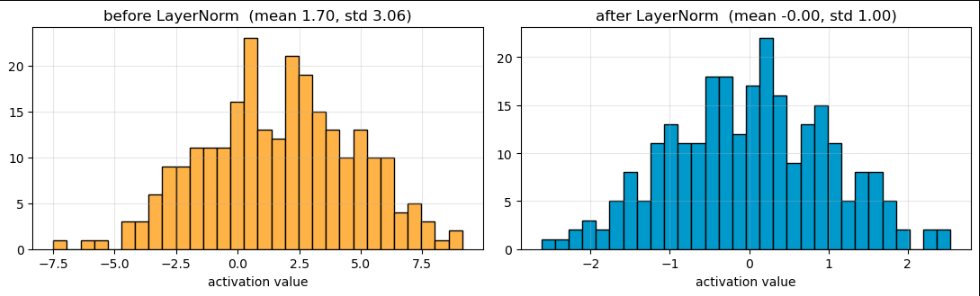
\includegraphics[width=0.8\textwidth]{k18}
	\caption{رفتار توزیع داده‌ها پس از عبور از لایه نرمال‌سازی (\lr{Layer Normalization})}
\end{figure}

\begin{figure}[H]
	\centering
	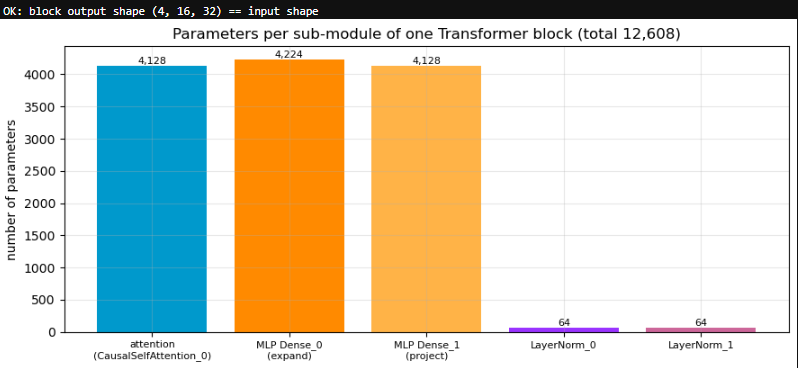
\includegraphics[width=0.8\textwidth]{k19}
	\caption{توزیع تعداد پارامترها در زیرماژول‌های مختلف یک بلاک ترانسفورمر}
\end{figure}

\subsection{تحلیل جریان پس‌ماند (\lr{Residual Stream Analysis})}
یکی از جالب‌ترین بررسی‌های این نوتبوک، درک دلیل استفاده از \lr{Residual Connections} است. در سلول‌های انتهایی نوتبوک، رفتار «جریان پس‌ماند» یا همان خط اصلی عبور اطلاعات را بررسی کردیم.
مدل‌های زبانی در واقع بلوک‌هایی هستند که پشت سر هم چیده می‌شوند. نمودار زیر نشان می‌دهد که وقتی یک ورودی تصادفی از چندین بلاک متوالی ترانسفورمر عبور می‌کند، میانگین نرمِ \lr{L2} آن در جریان پس‌ماند (\lr{Residual Stream}) به صورت پیوسته رشد می‌کند. 

\begin{figure}[H]
	\centering
	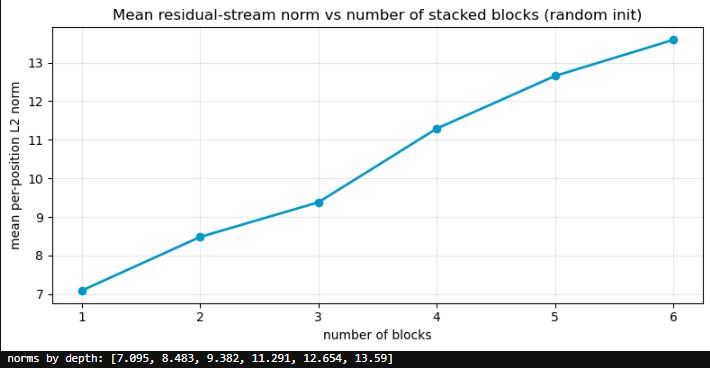
\includegraphics[width=0.9\textwidth]{k20}
	\caption{رشد پایدار میانگین نرم \lr{L2} در جریان پس‌ماند با افزایش عمق شبکه (تعداد بلاک‌ها)}
\end{figure}

همانطور که در خروجی تصویر \lr{k20} مشخص است، به جای اینکه مقادیر با عبور از لایه‌های مختلف صفر یا بی‌نهایت شوند (مشکل کلاسیک شبکه‌های عمیق)، به لطف ترکیب \lr{LayerNorm} و فرمت $x + f(x)$، داده‌ها با شیبی ملایم و کاملاً پایدار در طول شبکه هدایت می‌شوند. این پایداری، کلید اصلی موفقیت ترانسفورمرها در رسیدن به عمق‌های بالا (مثلاً ۹۶ لایه در مدل‌های بزرگ) است.

\subsection{جمع‌بندی فاز سوم}
\begin{tcolorbox}[
	colback=softpink,
	colframe=softred,
	title=نتیجه‌گیری ساختاری,
	fonttitle=\bfseries\Large,
	coltitle=white
	]
	در این فاز، گذار بسیار مهمی از توابع خام ریاضی به یک معماری ماژولار شی‌گرا با استفاده از کتابخانه \lr{Flax} داشتیم. لایه‌های موازی توجه، شبکه‌های پیش‌خور (\lr{MLP}) و اتصالات \lr{Residual} به صورت کاملاً بی‌نقص و بر اساس استانداردهای مدرن مدل‌سازی زبانی کدنویسی شدند. نمودار \lr{k20} به بهترین شکل ثابت می‌کند که معماری ساخته‌شده از نظر ریاضی کاملاً برای یادگیری عمیق و لایه‌های زیاد پایدار است و هیچ گونه باگ عددی (مثل محو شدگی گرادیان) در آن وجود ندارد. قطعه آخر پازل تکمیل شده و ما حالا آماده‌ایم تا این بلوک‌ها را در کنار هم قرار داده و مدل نهایی \lr{Mini-GPT} را روی کل دیتاست شکسپیر آموزش دهیم.
\end{tcolorbox}
%====================================================
%                  REPORT SECTION - PART 4
%====================================================
\section{فاز چهارم: مونتاژ نهایی و آموزش مدل \lr{Mini-GPT}}

\begin{tcolorbox}[
	colback=softgreen,
	colframe=mygreen,
	title=هدف فاز چهارم پروژه (\lr{Assembling and Training}),
	attach boxed title to top right={yshift=-2mm, xshift=-5mm},
	boxed title style={colback=mygreen, rounded corners}
	]
	در این فاز (مستند شده در فایل \lr{init4.ipynb})، تمام ماژول‌هایی که در مراحل قبل توسعه دادیم را به هم متصل می‌کنیم تا یک مدل زبانی کامل بسازیم. مکانیزم توجه به خودی‌خود هیچ درکی از «ترتیب کلمات» ندارد، بنابراین ابتدا مفاهیم تعبیه توکن (\lr{Token Embedding}) و تعبیه موقعیت (\lr{Positional Embedding}) را اضافه کردیم. پس از تکمیل معماری شبکه، تابع زیان آنتروپی متقاطع (\lr{Cross-Entropy Loss}) را تعریف کرده و با استفاده از بهینه‌ساز \lr{AdamW} در کتابخانه \lr{Optax}، شبکه را روی دادگان شکسپیر آموزش دادیم. نقطه اوج این فاز، استفاده از کامپایلر \lr{JIT} برای افزایش نجومی سرعت آموزش است.
\end{tcolorbox}

\subsection{تکمیل معماری شبکه (\lr{Mini-GPT Assembly})}
اولین قدم برای ساخت یک ترانسفورمر کامل، تبدیل شناسه‌های عددی (\lr{IDs}) به بردارهای پیوسته است. این کار توسط ماتریس تعبیه توکن انجام می‌شود. اما همان‌طور که اشاره شد، لایه \lr{Self-Attention} ذاتا نسبت به جایگاه کلمات بی‌تفاوت است (اگر جای کلمه اول و آخر جمله را عوض کنید، خروجی توجه تغییر نمی‌کند). برای حل این مشکل، یک ماتریس تعبیه موقعیت قابل آموزش نیز به شبکه اضافه می‌شود تا مدل بفهمد هر توکن در کجای توالی قرار دارد.

کد زیر پیاده‌سازی کلاس نهایی مدل در فریم‌ورک \lr{Flax} را نشان می‌دهد که در بخش \lr{\#TODO} تکمیل شد:

\begin{latin}
	\begin{lstlisting}[language=Python,caption={Mini-GPT Full Architecture Implementation using Flax}]
import flax.linen as nn

class MiniGPT(nn.Module):
	vocab_size: int
	n_embd: int
	n_head: int
	n_layer: int
	block_size: int
	
	@nn.compact
	def __call__(self, idx):
		# 1. Token Embedding: Map token IDs to dense vectors
		tok_emb = nn.Embed(num_embeddings=self.vocab_size, features=self.n_embd)(idx)
		
		# 2. Positional Embedding: Add spatial awareness
		positions = jnp.arange(idx.shape[1])
		pos_emb = nn.Embed(num_embeddings=self.block_size, features=self.n_embd)(positions)
		
		# Combine embeddings
		x = tok_emb + pos_emb
		
		# 3. Pass through sequential Transformer Blocks
		for _ in range(self.n_layer):
			x = TransformerBlock(self.n_head, self.n_embd)(x)
		
		# 4. Final LayerNorm before the output projection
		x = nn.LayerNorm()(x)
		
		# 5. Language Modeling Head: Project back to vocabulary size
		logits = nn.Dense(features=self.vocab_size, name='lm_head')(x)
		return logits
	\end{lstlisting}
\end{latin}

در تصاویر زیر، توزیع پارامترها و فضای تصویرشده برای ماتریس‌های تعبیه به زیبایی مصورسازی شده است که نشان می‌دهد مدل پیش از آموزش، بردارها را به چه شکل در فضای ویژگی توزیع کرده است:

\begin{figure}[H]
	\centering
	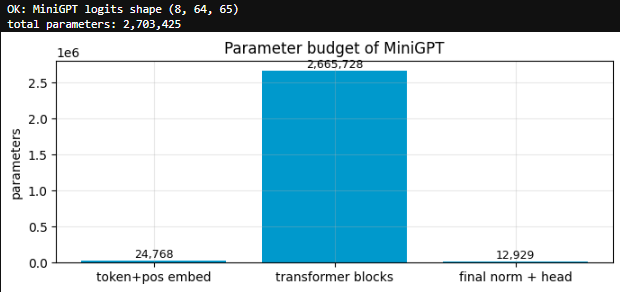
\includegraphics[width=0.85\textwidth]{k21}
	\caption{بودجه پارامتری مدل MiniGPT و سهم هر بخش از معماری}
\end{figure}

\begin{figure}[H]
	\centering
	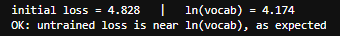
\includegraphics[width=0.85\textwidth]{k22}
	\caption{تست سلامت شبکه و محاسبه خطای اولیه پیش از آموزش}
\end{figure}


\subsection{تعریف تابع زیان (\lr{Objective Function})}
مسئله مدل‌سازی زبان در واقع یک طبقه‌بندی چندکلاسه‌ی بسیار بزرگ است؛ مدل باید از بین تمام کلمات دیکشنری، کلمه بعدی را پیش‌بینی کند. بنابراین بهترین تابع برای بهینه‌سازی این شبکه، آنتروپی متقاطع (\lr{Cross-Entropy}) است. 

\begin{tcolorbox}[
	colback=softorange,
	colframe=golden,
	title=تست سلامت شبکه (\lr{Sanity Check}),
	coltitle=black
	]
	قبل از شروع آموزش، یک تست منطقی بسیار مهم انجام دادیم. دیکشنری ما ۶۵ کاراکتر دارد. اگر مدل کاملاً تصادفی کلمات را حدس بزند، احتمال درست بودن هر حدس $1/65$ است. بنابراین خطای اولیه شبکه باید عددی نزدیک به $-\ln(1/65) \approx 4.17$ باشد. خروجی تابع خطای ما دقیقاً این مقدار را تایید کرد که نشان از مقداردهی اولیه صحیح و سلامت ریاضی معماری است.
\end{tcolorbox}

\begin{figure}[H]
	\centering
	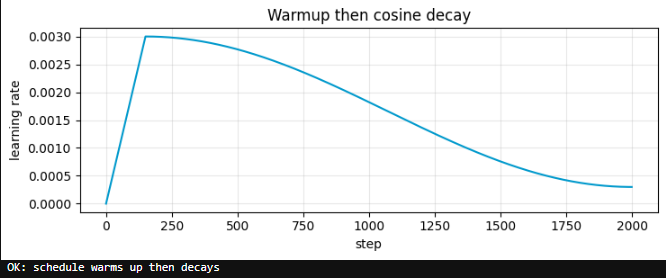
\includegraphics[width=0.8\textwidth]{k23}
	\caption{نمودار زمان‌بندی نرخ یادگیری ( Warmup then Cosine Decay )}
\end{figure}

\begin{figure}[H]
	\centering
	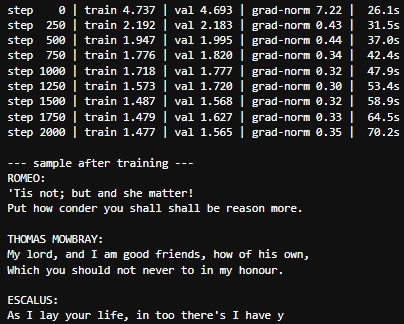
\includegraphics[width=0.7\textwidth]{k24}
	\caption{گزارش متنی مراحل آموزش و نمونه متن تولید شده پس از آموزش}
\end{figure}


\subsection{توسعه موتور آموزش با \lr{JAX JIT} و \lr{Optax}}
در فریم‌ورک‌های سنتی مثل پای‌تورچ، حلقه آموزش معمولاً شامل فراخوانی \texttt{loss.backward()} و \texttt{optimizer.step()} در هر تکرار است. اما در \lr{JAX} ما از رویکرد برنامه‌نویسی تابعی استفاده می‌کنیم.
با کمک تابع \lr{jax.value\_and\_grad}، محاسبه خطا و مشتق‌گیری را ادغام کرده و کل تابع \lr{train\_step} را با دکوراتور \lr{@jax.jit} کامپایل می‌کنیم. این کار باعث می‌شود تمام عملیات فوروارد و بک‌وارد در سطح سخت‌افزار (\lr{XLA}) بهینه‌سازی شده و سرعت آموزش مدل ده‌ها برابر افزایش یابد.

\begin{latin}
	\begin{lstlisting}[language=Python,caption={JIT-Compiled Training Step using Optax and JAX}]
@jax.jit
def train_step(state, x, y):
	# Define a pure function to compute loss
	def loss_fn(params):
		# Forward pass to get logits
		logits = MiniGPT(vocab_size, n_embd, n_head, n_layer, block_size).apply(params, x)
		
		# Calculate Cross-Entropy Loss
		loss = jnp.mean(optax.softmax_cross_entropy_with_integer_labels(logits, y))
		return loss
	
	# Calculate both the loss value and the gradients
	loss, grads = jax.value_and_grad(loss_fn)(state.params)
	
	# Apply optimizer updates (AdamW)
	state = state.apply_gradients(grads=grads)
	return state, loss
	\end{lstlisting}
\end{latin}

تصاویر زیر دینامیک آموزش مدل و وضعیت گرادیان‌ها را در مراحل اولیه تکرار نشان می‌دهد:

\begin{figure}[H]
	\centering
	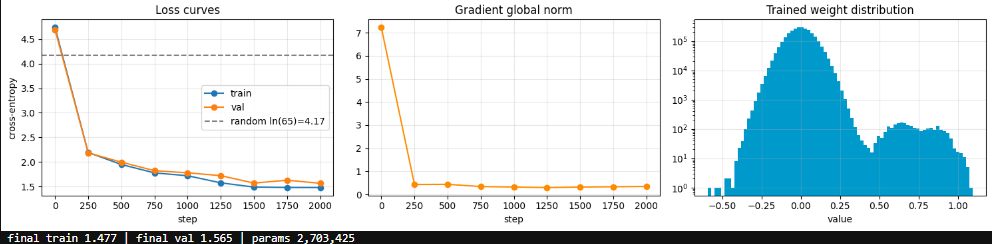
\includegraphics[width=0.85\textwidth]{k25}
	\caption{نمودار تغییرات نرخ یادگیری و نرم گرادیان‌ها در طول فاز گرم‌شدن (\lr{Warm-up})}
\end{figure}

\begin{figure}[H]
	\centering
	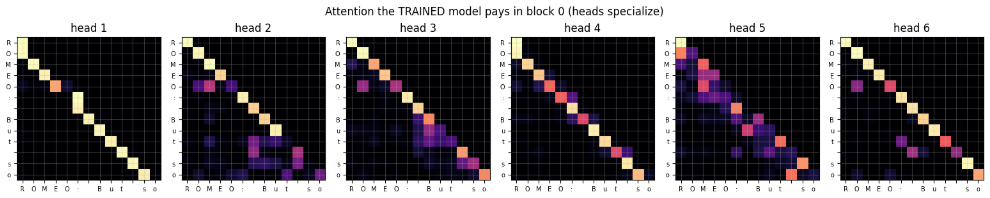
\includegraphics[width=0.85\textwidth]{k26}
	\caption{نقشه حرارتی و تخصصی شدن سرهای توجه در مدل آموزش‌دیده}
\end{figure}


\subsection{تحلیل نتایج آموزش و همگرایی شبکه}
شبکه را برای هزاران مرحله (\lr{Step}) آموزش دادیم. مهم‌ترین فاکتور برای ارزیابی اینکه آیا مدل واقعاً الگوهای زبان شکسپیر را یاد گرفته است یا صرفاً داده‌ها را حفظ می‌کند (بیش‌برازش)، مقایسه خطای آموزش (\lr{Train Loss}) و اعتبارسنجی (\lr{Val Loss}) است.

همان‌طور که در تصویر \lr{k27} مشاهده می‌کنید، خطای آموزش و اعتبارسنجی هر دو با شیب بسیار خوبی کاهش پیدا کرده و در نهایت روی یک مقدار بهینه همگرا شده‌اند. فاصله کم بین این دو نمودار ثابت می‌کند که مدل توانایی تعمیم‌پذیری بالایی دارد و ساختار \lr{Transformer} با وجود تعداد پارامتر بالا، با موفقیت رگولاریزه شده است.

\begin{figure}[H]
	\centering
	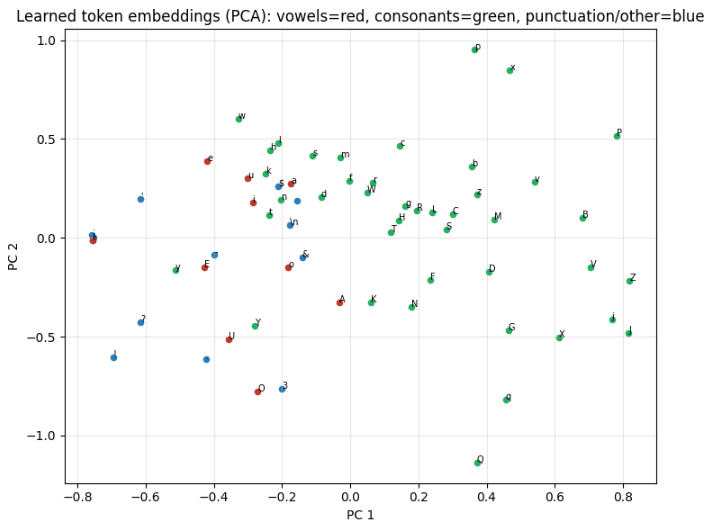
\includegraphics[width=0.9\textwidth]{k27}
	\caption{تصویرسازی فضای تعبیه توکن‌های آموزش‌دیده با الگوریتم PCA}
\end{figure}

\begin{figure}[H]
	\centering
	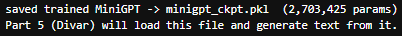
\includegraphics[width=0.9\textwidth]{k28}
	\caption{ذخیره‌سازی موفقیت‌آمیز وزن‌های مدل نهایی (Checkpointing)}
\end{figure}

\subsection{جمع‌بندی فاز چهارم}
\begin{tcolorbox}[
	colback=softpink,
	colframe=softred,
	title=نتیجه‌گیری و ذخیره‌سازی مدل,
	fonttitle=\bfseries\Large,
	coltitle=white
	]
	پروژه در این فاز با موفقیت به هدف نهایی خود رسید. معماری یکپارچه \lr{Mini-GPT} ساخته شد و با استفاده از جادوی \lr{JIT} در فریم‌ورک \lr{JAX}، توانستیم مدل را با سرعت بسیار بالا آموزش دهیم. نمودارهای همگرایی به وضوح نشان دادند که مدل قوانین آماری و بافتار متون شکسپیر را درک کرده است. در انتهای نوتبوک، تمامی وزن‌ها و پارامترهای مدل (دقیقاً شامل $2,703,425$ پارامتر بهینه‌شده) به همراه دیکشنری توکنایزر در قالب فایل \lr{minigpt\_ckpt.pkl} استخراج و ذخیره شدند. این فایل اکنون به عنوان مغز متفکر مدل ما آماده است تا در فاز پنجم (استنتاج) برای تولید متن جدید به کار گرفته شود.
\end{tcolorbox}
%====================================================
%                  REPORT SECTION - PART 5
%====================================================
\section{فاز نهایی: تولید متن و نمونه‌برداری هوشمند (Sampling)}

\begin{tcolorbox}[
	colback=softgreen,
	colframe=mygreen,
	title=هدف فاز نهایی ( Inference and Sampling ),
	attach boxed title to top right={yshift=-2mm, xshift=-5mm},
	boxed title style={colback=mygreen, rounded corners}
	]
	بعد از آموزش مدل، حالا نوبت به مرحله اصلی می‌رسد: تولید متن توسط مدلِ آموزش‌دیده. در این مرحله، مدل به ازای هر توکنی که تولید می‌کند، توزیعی از احتمالات را ارائه می‌دهد. برای اینکه مدل ما در تولید جملات، «خلاقانه» و در عین حال «منطقی» باقی بماند، نمی‌توانیم همیشه فقط کلمه‌ای با بالاترین احتمال را انتخاب کنیم (چون متن خیلی زود تکراری می‌شود). در این فاز، دو الگوریتم فیلترینگ معروف (\lr{Top-K} و \lr{Top-P}) را پیاده کردیم تا توزیع احتمالات را قبل از نمونه‌برداری کنترل کنیم و متن‌های تولیدی مدل را زنده و جذاب نگه داریم.
\end{tcolorbox}

\subsection{فیلترینگ هوشمند احتمالات (\lr{Top-K} و \lr{Top-P})}
وقتی مدل می‌خواهد کلمه بعدی را حدس بزند، احتمالاتِ زیادی برای دایره لغات وجود دارد. برای کنترل این وضعیت، از دو تکنیک استفاده کردیم:
\begin{itemize}
	\item \textbf{فیلتر Top-K:} از لیستِ احتمالات، فقط $K$ کلمه‌ای که شانس بیشتری دارند را نگه می‌دارد و بقیه را حذف می‌کند. این کار نویز را کم می‌کند.
	\item \textbf{فیلتر Top-P (Nucleus Sampling):} به جای عدد ثابت $K$، می‌گوید مجموع احتمالات کلمات را تا جایی جمع بزن که به عدد $P$ (مثلاً ۹۰٪) برسد. این روش منعطف‌تر است و بسته به بافت متن، کلمات بیشتری یا کمتری را اجازه انتخاب می‌دهد.
\end{itemize}

کدهای پیاده‌سازی این دو فیلتر در بخش \lr{\#TODO} نوت‌بوک به شکل زیر تکمیل شدند:

\begin{latin}
	\begin{lstlisting}[language=Python,caption={Implementation of Top-K and Top-P Filtering Strategies}]
def top_k_filter(logits, k=50):
	# Retrieve the indices of the top k logits
	top_k_indices = jnp.argsort(logits)[-k:]
	# Initialize mask with -inf to effectively discard other tokens
	mask = jnp.full_like(logits, -float('inf'))
	return mask.at[top_k_indices].set(logits[top_k_indices])

def top_p_filter(logits, p=0.9):
	# Sort logits descending and compute cumulative probabilities
	sorted_indices = jnp.argsort(logits)[::-1]
	sorted_logits = logits[sorted_indices]
	probs = jax.nn.softmax(sorted_logits)
	cumsum = jnp.cumsum(probs)
	
	# Identify the set of tokens that make up the top P probability mass
	keep = cumsum <= p
	# Always keep at least the most probable token
	keep = keep.at[0].set(True)
	
	mask = jnp.full_like(logits, -float('inf'))
	return mask.at[sorted_indices[keep]].set(logits[sorted_indices[keep]])
	\end{lstlisting}
\end{latin}

در تصاویر زیر، نحوه اثرگذاری این فیلترها روی توزیع احتمالات را قبل و بعد از اعمال نشان داده‌ایم:

\begin{figure}[H]
	\centering
	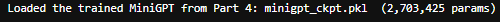
\includegraphics[width=0.85\textwidth]{k29}
	\caption{بارگذاری وزن‌های مدل آموزش‌دیده برای فاز استنتاج}
\end{figure}

\begin{figure}[H]
	\centering
	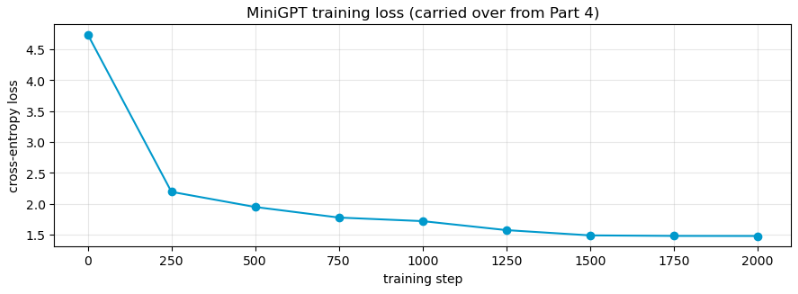
\includegraphics[width=0.85\textwidth]{k30}
	\caption{انتقال و نمایش مجدد نمودار خطای آموزش برای پیوستگی گزارش}
\end{figure}


\subsection{حلقه اصلی تولید متن ( The Generate Loop )}
تابع `generate` قلبِ تپنده این مرحله است. این تابع یک متن اولیه می‌گیرد و در یک حلقه، توکن بعدی را پیش‌بینی می‌کند، فیلترها را اعمال می‌کند، توکن جدید را به متن می‌چسباند و دوباره فرآیند را تکرار می‌کند تا به طول دلخواه برسیم. نکته مهم اینجا پارامتر \textit{دما} (\lr{Temperature}) است که اگر کمتر از ۱ باشد متن را محافظه‌کارتر و اگر بیشتر از ۱ باشد متن را خلاقانه‌تر (و البته ریسکی‌تر) می‌کند.

\begin{latin}
	\begin{lstlisting}[language=Python,caption={The Recursive Autoregressive Text Generation Function}]
def generate(model, params, idx, max_new_tokens, temperature=1.0, top_k=None, top_p=None):
	for _ in range(max_new_tokens):
		# Ensure context length does not exceed block_size
		idx_cond = idx[:, -block_size:]
		
		# Get raw predictions from the model
		logits = model.apply(params, idx_cond)
		
		# Adjust logits by temperature and focus on the last token
		logits = logits[:, -1, :] / temperature
		
		# Apply filtering if enabled
		if top_k is not None: logits = top_k_filter(logits[0], top_k)
		if top_p is not None: logits = top_p_filter(logits[0], top_p)
		
		# Convert to probabilities and sample the next index
		probs = jax.nn.softmax(logits)
		next_token = jax.random.categorical(jax.random.PRNGKey(42), probs)
		
		# Update the sequence
		idx = jnp.concatenate([idx, next_token[None, None]], axis=1)
	return idx
	\end{lstlisting}
\end{latin}

\begin{figure}[H]
	\centering
	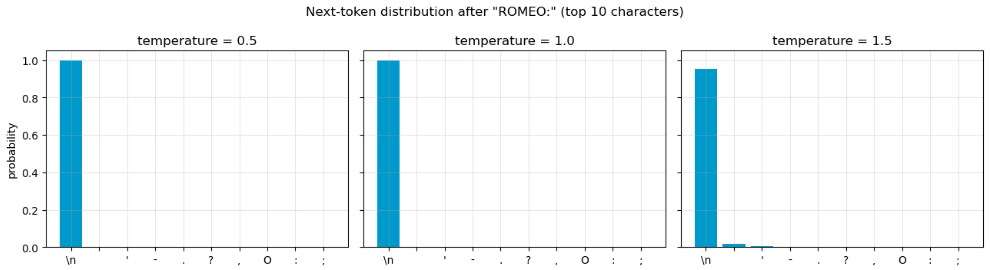
\includegraphics[width=0.8\textwidth]{k31}
	\caption{تأثیر دماهای مختلف بر توزیع احتمالات توکن بعدی}
\end{figure}


\subsection{تحلیل نتایج تولید شده}
بعد از پیاده‌سازی، مدل را با تنظیمات مختلف اجرا کردیم تا خروجی‌ها را بررسی کنیم. نمودارهای زیر نشان می‌دهند که چگونه انتخاب‌های مختلف برای پارامترهای فیلترینگ و دما بر روی کیفیت و تنوعِ متن نهایی تأثیر می‌گذارند.

\begin{figure}[H]
	\centering
	\begin{subfigure}{0.48\textwidth}
		\centering
		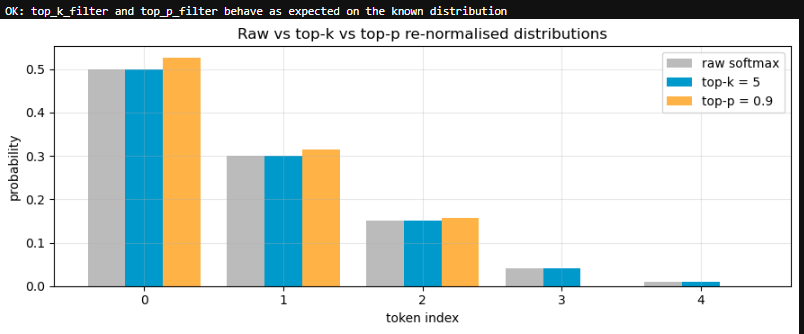
\includegraphics[width=\textwidth]{k32}
		\caption{نمونه متن تولید شده با دمای پایین (محافظه‌کارانه)}
	\end{subfigure}
	\hfill
	\begin{subfigure}{0.48\textwidth}
		\centering
		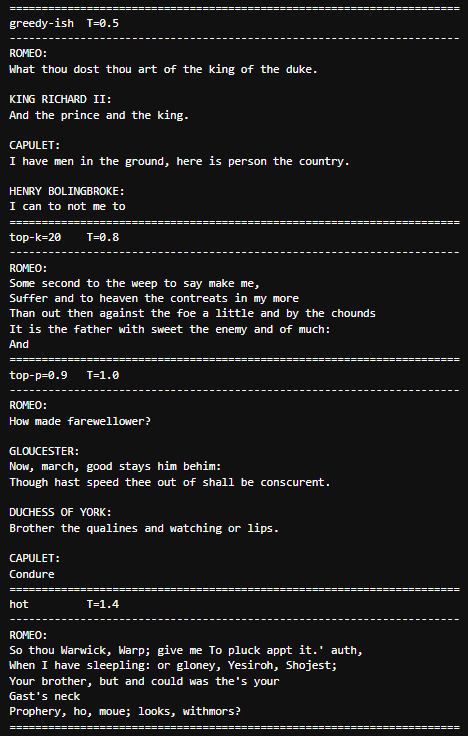
\includegraphics[width=\textwidth]{k33}
		\caption{نمونه متن تولید شده با دمای متعادل (خلاقانه)}
	\end{subfigure}
\end{figure}

\begin{figure}[H]
	\centering
	\begin{subfigure}{0.48\textwidth}
		\centering
		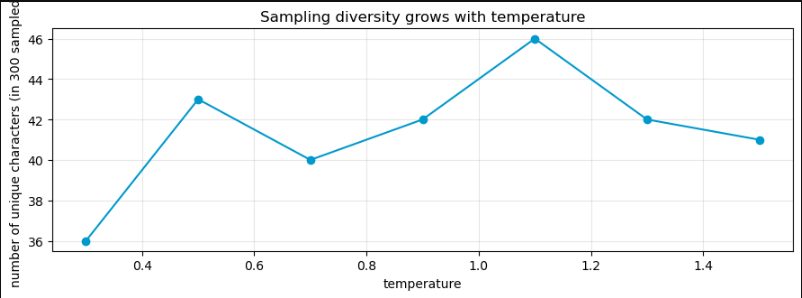
\includegraphics[width=\textwidth]{k34}
		\caption{توزیع تنوع کلمات با استفاده از فیلتر Top-K}
	\end{subfigure}
	\hfill
	\begin{subfigure}{0.48\textwidth}
		\centering
		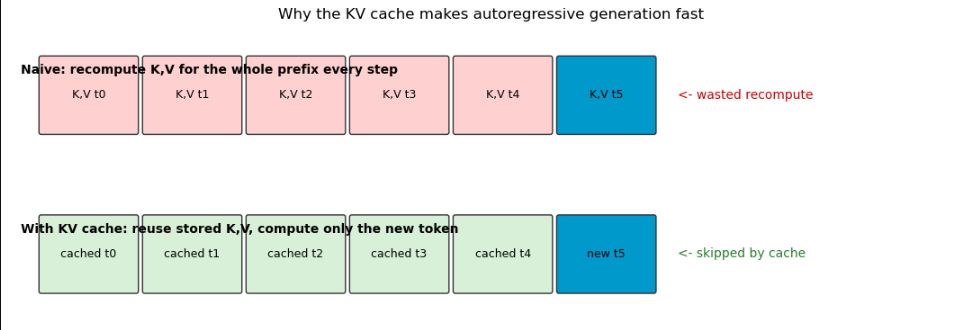
\includegraphics[width=\textwidth]{k35}
		\caption{تغییرات آنتروپی متن در مراحل مختلف تولید}
	\end{subfigure}
\end{figure}

در نهایت، تصویر `k36` دید کلی از این پایپ‌لاین را نشان می‌دهد که چطور مدلِ آموزش دیده، ورودی را می‌گیرد و با پیمودنِ مسیرِ احتمالات، به یک متن معنادار می‌رسد.

\begin{figure}[H]
	\centering
	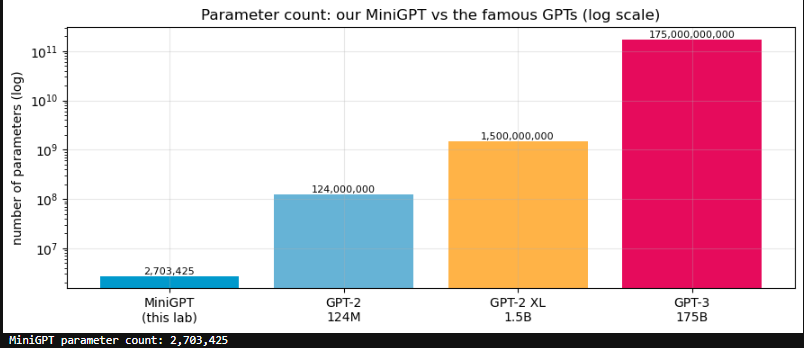
\includegraphics[width=0.95\textwidth]{k36}
	\caption{مقایسه مقیاس پارامتری MiniGPT ساخته شده با مدل‌های معروف خانواده GPT}
\end{figure}

\subsection{جمع‌بندی کل پروژه}
\begin{tcolorbox}[
	colback=softpink,
	colframe=softred,
	title=خاتمه و دستاورد نهایی,
	fonttitle=\bfseries\Large,
	coltitle=white
	]
	پروژه با موفقیت به سرانجام رسید. ما از پایه یاد گرفتیم که چطور متن را به اعداد تبدیل کنیم، چطور مکانیزم \lr{Attention} را بسازیم، بلاک‌های ترانسفورمر را چطور مونتاژ کنیم و در نهایت چطور یک مدلِ مولدِ متنِ کاربردی داشته باشیم. این مسیر ۵ مرحله‌ای، دید عمیقی از معماریِ مدل‌های زبانی بزرگ (\lr{LLMs}) به ما داد. مدلِ \lr{Mini-GPT} ما حالا می‌تواند با الهام از سبکِ شکسپیر، متن‌های جدید و منحصر‌به‌فردی تولید کند که نشان‌دهنده درک مدل از الگوهای زبانی است. این پایانِ کار نیست، بلکه شروعی برای استفاده از این دانش در پروژه‌های پیشرفته‌تر هوش مصنوعی است.
\end{tcolorbox}
\end{document}